\section{ODE solvers} 

ODE solvers implement animation algorithms applied at each time step to integrate time and compute positions and velocities one time step forward in time.
% Each step of the algorithm is implemented using a visitor to traverse the scenegraph starting from the node the solver is attached to.
The solvers do not directly address the physical models. 
They apply abstract mechanical operations to state vectors represented by IDs, as illustrated in the algorithm shown in Figure~\ref{fig:eulerexplicit}.
\begin{figure}
\begin{center}
\begin{algorithmic}
\STATE void  \textbf{ExplicitEulerSolver::solve(VecId x, VecId v, double dt)}
\STATE create auxiliary vectors a,f
\STATE resetForce(f)
\STATE accumulateForce(f,x,v)
\STATE computeAcceleration(a,f)
\STATE project(a,a)
\STATE v += a * dt
\STATE x += v * dt
\end{algorithmic}
\caption{Euler's explicit time integration.}
\label{fig:eulerexplicit}
\end{center}
\end{figure}
Each mechanical operation, such as allocating a state vector or accumulating the forces, is implemented using a specialized visitor parameterized on vector IDs or control values such as dt.
This allows to implement the solvers completely independenly of the physical model.
Each vector used by a solver ID is actually scattered over all the state vector containers in the different nodes in the scope of the solver.
Some vector operations such as the dot product apply only to the independent DOFs, stored in the state vectors not attached to a parent by a mapping.
Notice that this design avoids the assembly of global state vectors (i.e. copying Vec3 and quaternions to and from  vectors of scalars).
Moreover, the virtual function calls are resolved at the granularity of the state vectors (i.e. all the particles together, and all the moving frames together) rather than each primitive (i.e. each particle and each frame independently), and allow to optimize each implementation independently.
There is thus virtually no loss of efficiency when mixing arbitrary types in the same simulation.




% The ODE solver creates visitors and applies them to its parent node.
% The ComputeDf visitor presented in Figure~\ref{fig:DfVisitor} finds no mapping nor DOF at the root level (functions are called only if the corresponding component is present in the node), and continues the traversal in the two child branches. 
% Each object computes its own force change df corresponding to its own displacement dx, as previously explained.
% The objects are independent because there is no mapping to a commom DOF component at the scene level.
% Each object manages its own state vectors.
% Thus, using visitors allows the solver to transparently handle an arbitrary number of objects of arbitrary types in the same scene. 
% One can use visitors without knowing to which objects they apply.
% This is a key feature of the SOFA design, which allows us design the algorithms once and to apply them to all types of simulated objects.
% Notice that this design avoids the assembly of global state vectors (i.e. copying Vec3 and quaternions to and from  vectors of scalars).
% Moreover, the virtual function calls are resolved at the granularity of the state vectors (i.e. all the particles together, and all the moving frames together) rather than each primitive (i.e. each particle and each frame independently), and allow to optimize each implementation independently.
% There is thus virtually no loss of efficiency when mixing arbitrary types in the same simulation.
% Hence the ``versatile yet efficient'' motto of SOFA.


We have identified two families of ODE solvers.
The first contains the explicit solvers, which compute the derivative at the beginning of the time step. They are variants of the Euler explicit solver presented in Figure~\ref{fig:eulerexplicit}, and are easily implemented in Sofa using the same operators.
The second family contains the implicit solvers, which consider the derivative at the end or somewhere in the middle of the time step. They typically require the solution of equation systems such as:
\begin{equation}
\label{eq:linear-system}
\underbrace{\left(\alpha \M  + \beta \B  + \gamma \K \right)}_{\mathbf{A}}   \Vdv =  \vec b
%\underbrace{\P \left(\alpha \M  + \beta \B  + \gamma \K \right)}_{\mathbf{A}}   \Vdv =  \vec b
\end{equation}
where $\M$ is the mass matrix, $\K = \frac{\partial \Vf}{\partial \Vx}$ and $\B = \frac{\partial \Vf}{\partial \Vv}$ respectively are the \textit{stiffness} and \textit{damping} matrices (the method is explicit if $\beta$ and $\gamma$ are null). In order to apply simple displacement constraints,  a projection matrix $\P$ can be used, and the system becomes $\P^T \mathbf{A} \P \Vdv =\P^T \vec b $~\cite{baraff98large}.
Implicit integration has the advantage of being more stable for stiff forces or large time steps. However, solving these equation systems requires linear solvers, discussed in the next section.
Currently, eight ODE solvers have been implemented, including symplectic Euler and explicit Runge-Kutta4, implicit Euler and statics solution.



\section{Linear solvers} 
\subsection{Conjugate Gradient} An interesting feature of visitor-based mechanical computations is their ability to efficiently and transparently compute matrix products.
Thus, we have proposed in SOFA an implementation of the Conjugate Gradient, based on the graph traversal. 
The visitor shown in Figure~\ref{fig:DfVisitor} computes the force change \textit{df} based on a given displacement \textit{dx}, as repeatedly performed in Conjugate Gradient algorithm. 
An arbitrary number of forces and projections may be present in all the nodes, resulting in a complicated stiffness matrix, as shown in the following equation:
\begin{equation}
 \label{eq:dfdx}
\vec{df} = \sum_i  \left( \prod_{j \in path(i)} \mat J_j  \right)^T \K_i \left( \prod_{j \in path(i)} \mat J_j  \right) \vec{dx}
\end{equation}
where $\K_i$ is the stiffness matrix of force $i$, matrix $\J$ encodes the first-order mapping relation of a node with respect to its parent, and $path(i)$ is the list of nodes from the solver to the node the force applies to.
\begin{figure}
\begin{center}
\begin{tabular}{c|c}
\begin{minipage}[t]{0.52\linewidth}
\begin{algorithmic}
\STATE bool \textbf{ComputeDfVisitor::topDown}():
\STATE dof.resetF(this.df)
\IF{mapping}
\STATE mapping.applyJ(this.dx)
\ENDIF
% \FORALL {projection P}
% \STATE P.project( this.dx,this.dx )
% \ENDFOR
\RETURN true
\end{algorithmic}
\end{minipage}
&
%  \hspace{0.01\linewidth}
% &
%  \hspace{0.01\linewidth}
% &
 \begin{minipage}[t]{0.46\linewidth}
\begin{algorithmic}
\STATE void \textbf{ComputeDfVisitor::bottomUp}():
\FORALL {forceField F}
\STATE F.addDF( this.df,this.dx )
\ENDFOR
% \FORALL {projection P}
% \STATE P.project( this.df,this.df )
% \ENDFOR
\STATE mapping.applyJT(this.df)
\end{algorithmic}
 \end{minipage}
\end{tabular}
\caption{Computing $df$ given $dx$ using a visitor.}
\label{fig:DfVisitor}
\end{center}
\end{figure}
This complex product is computed using only matrix-vector products and with optimal factoring thanks to the recursive implementation.
It allows us to efficiently apply implicit time integration to arbitrary scenes using the Conjugate Gradient. 
This method allows us to trade-off accuracy for speed by limiting the number of steps of the iterative solution.


\subsection{Direct Solvers} Direct solvers are also available in SOFA. They can be used as preconditionners of the conjugate gradient algorithm~\cite{CADC10} or for directly solving equation \ref{eq:linear-system}.
Their implementation are based on external libraries such as Eigen, MKL and Taucs. 
When dealing with Finite Element Models, the matrices are generally very sparse and 
efficient implementations based on sparse factorizations allow for fast computations. 
Moreover, when dealing with specific topologies, like wire-like structures, tri-diagonal band solvers can be used for extremely fast results in $\mathcal{O}(n)$
These different linear solvers address matrices which  can be stored in different formats, adapted to the numerical library.
%or even not explicitly stored when only matrix-vector products are applied.
The type of matrix is a parameter of the linear solver, and of the visitors the solver uses. 
Ten linear solvers have been implemented in \sofa{}. They can be interchanged to compare their efficiency.

\subsection{From ODE solver to linear solver}

In SOFA, all states of a mechanical object is described by its degree of freedom. The main works for the simulation are filling and inverting a matrix system in order to find the states of mechanical objects by steps of time. This system matrix can be described as below :
 \[
\left[ \textbf{MBK} \right].a=f \text{    ,  or at time n+1 :   }\left[ \textbf{MBK} \right].a_{n+1}=f_{n+1}
\]
where,
\[
\left\{ 
\begin{array}{l}
\textbf{M} \text { : the mass matrix   }  \\
\textbf{B} \text { : the damping matrix   }  \\
\textbf{K} \text { : the stiffness matrix   }  \\
\left[ \textbf{MBK} \right] \text {  : is a linear combination of MBK (not multiplication)   }  \\
a_{n+1} \text { : accelerator field} \\
f_{n+1} \text { : force field} 
\end{array}\right.
\]
 Usually, \textbf{M} is filled by \textbf{mass} components, \textbf{K} is filled by \textbf{forcefield} or \textbf{interactionforcefield} components, \textbf{B} (often $\alpha\textbf{M}+\beta\textbf{K}$ ) and $\left[ \textbf{MBK} \right]$ are computed by \textbf{odesolver} components. The works left to invert the matrix system are done by \textbf{linearsolver} components.
\begin{center}
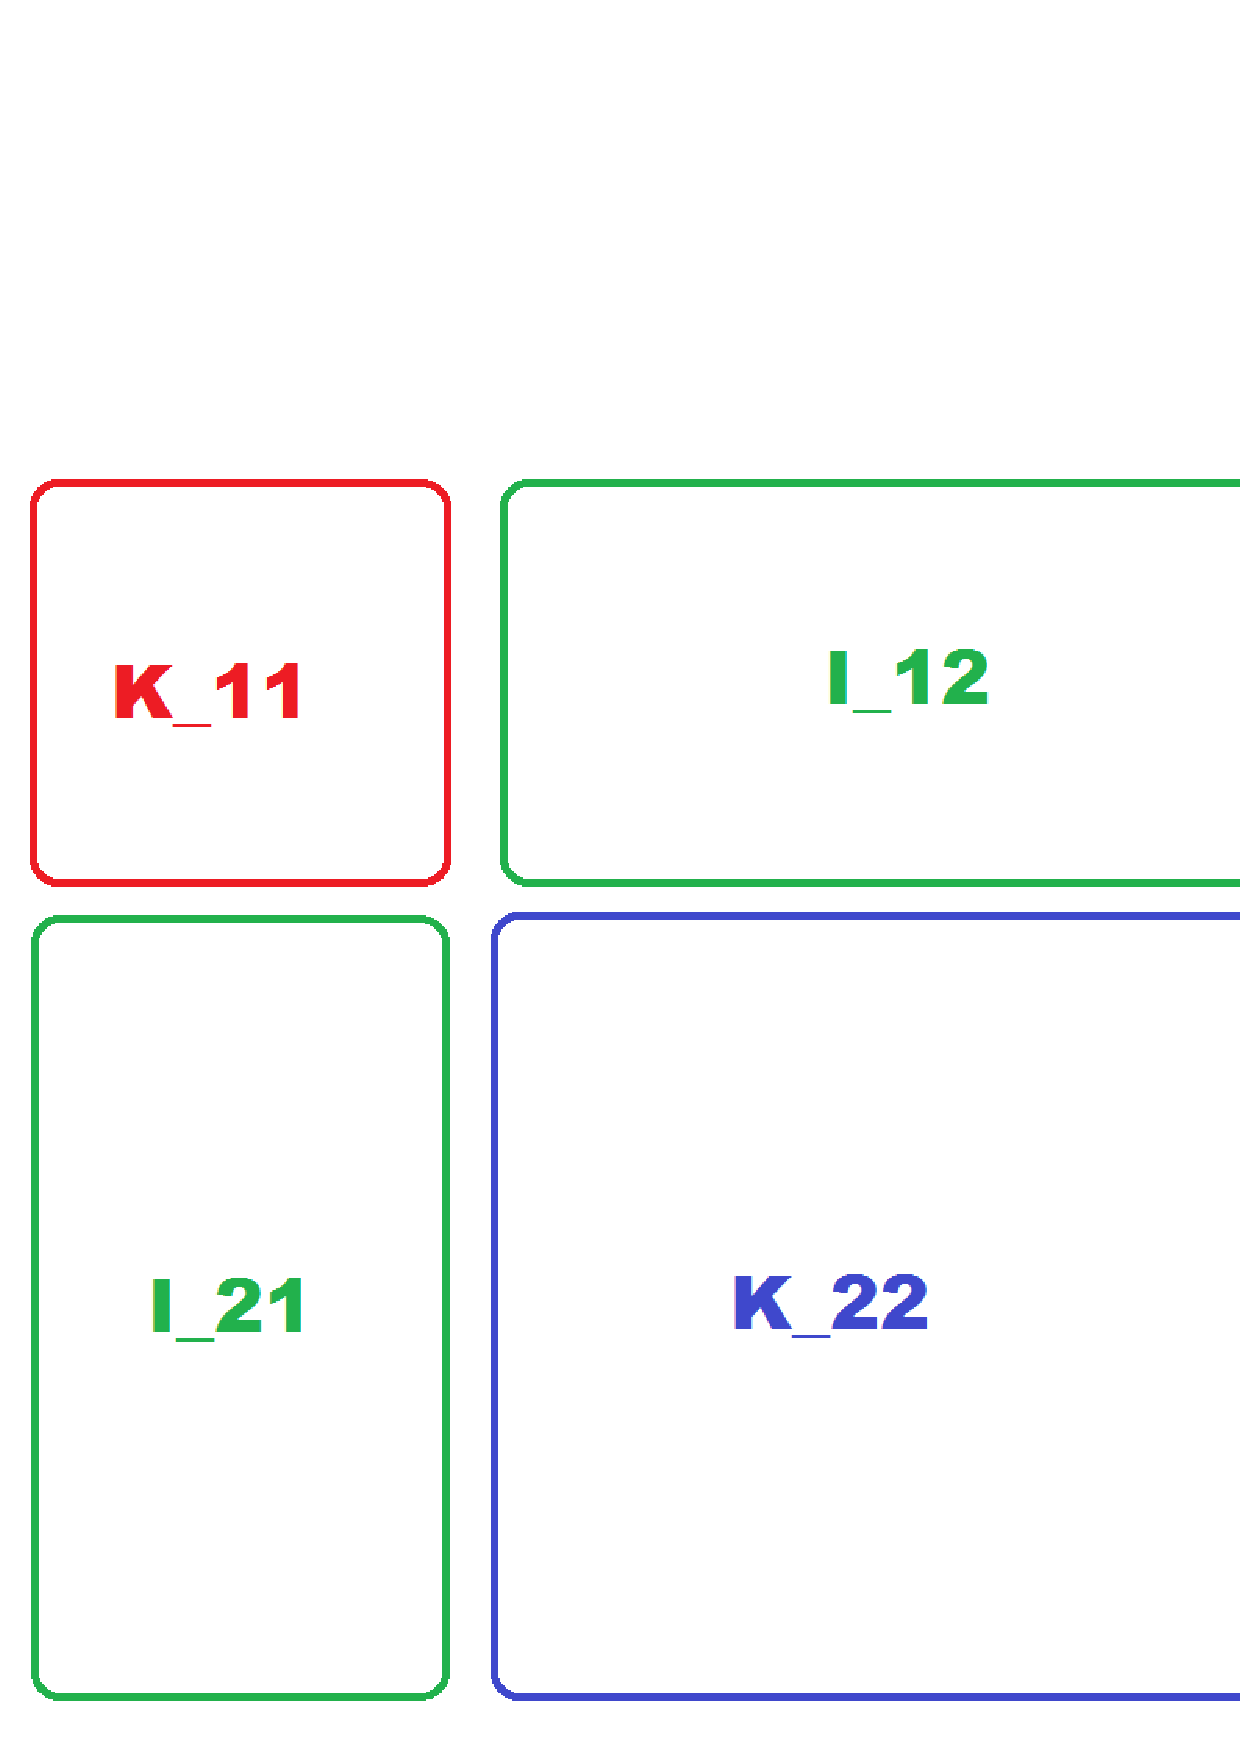
\includegraphics[scale=0.3]{matrix_bloc.pdf}
\end{center}
On the case for example when there are two mechanical objects, we can see a global stiffness matrix describing the two mechanical states, composed diagonal blocs and non-diagonal blocs. The diagonal blocs are filled by \textbf{mass},\textbf{forcefield} components, and the non-diagonal ones are filled by \textbf{interactionforcefield} if existed.
\paragraph{Mapping matrix contribution : } When existe a mapping on the simulation scene, the states of two mechanical objects are relied by : 
\[
\begin{array}{rl}
\textbf{x}_{2} & = \Im\left(\textbf{x}_{1}\right)           \text{      ,	mapping::apply}             \\
\textbf{v}_{2} & = \left[\textbf{J}\right] \textbf{v}_{1}   \text{      ,	mapping::applyJ}  
\end{array}
\]
The $\left[\textbf{J}\right]$ matrix is derivative of $\Im$ operator and is defined by the \textbf{mapping} components. The dynamic and matrix system of the two objects are relied by :   
\[
\begin{array}{rl}
\textbf{f}                  & += \textbf{f}_{1}  +   \left[\textbf{J}\right]^{t} \textbf{f}_{2}         \text{      ,	mapping::applyJT}             \\
\left[ \textbf{MBK} \right] & += \left[ \textbf{MBK} \right]_{1}  + \left[\textbf{J}\right]^{t}  \left[ \textbf{MBK} \right]_{2} \left[\textbf{J}\right]
\end{array}
\]
The resolution of the system with the mapping is done in general :
\[
\left\{ 
\begin{array}{rl}
\textbf{a}^{n+1}        & = \left[ \textbf{MBK} \right]^{-1}  \textbf{f}^{n+1}    \\
\textbf{v}^{n+1}_{1}    & = \textbf{v}^{n}_{1}     + dt.\textbf{a}^{n+1}         \\
\textbf{x}^{n+1}_{1}    & = \textbf{x}^{n}_{1}     + dt.\textbf{v}^{n+1}         \\
\textbf{x}^{n+1}_{2}    &  \text{ ,	mapping::apply }     \\
\textbf{v}^{n+1}_{2}    &  \text{ ,	mapping::applyJ }          
\end{array}
\right.
\]



\subsection{Particular implementation in SOFA}
The direct solver demands to build explicitly the matrix, and invert this matrix after every step of time in order to solve the mechanical response after a solicitation. In SOFA, there are a little more complicated component called mapping, relying geometrical and mechanical properties by master-slave (DOF-mapped object) relation. All changes of geometry or solicitation to one object interfere to other and vice versa. If the mapped object have its own mechanical behavior, it must be counted on the mechanical propagation by the mapping.
\subsubsection{self-stiffness propagation }
\[
\begin{array}{cc}
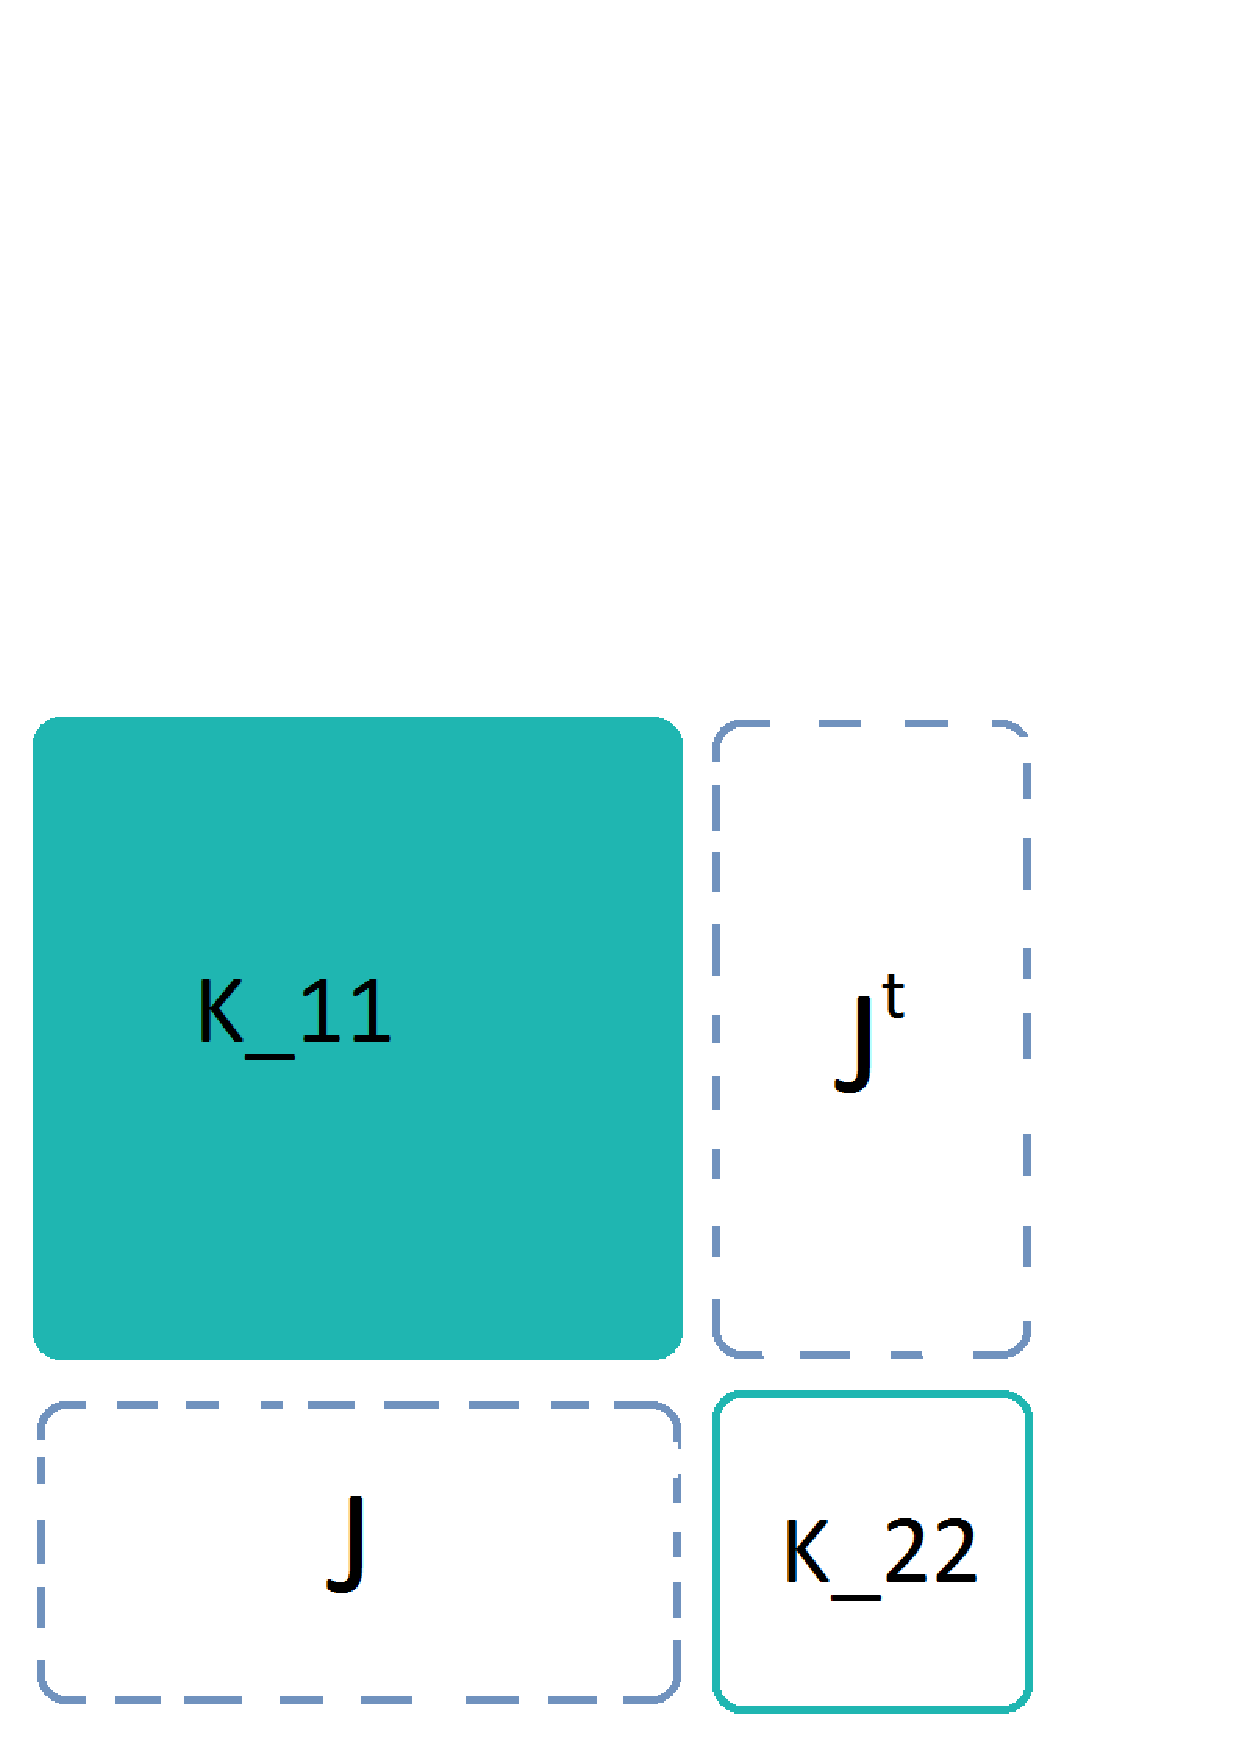
\includegraphics[scale=0.3]{stiffness_propagation_matrix.pdf}        
& 
\includegraphics[scale=0.35]{stiffness_propagation.pdf} 
\end{array}
\]
In the simple simulation scene, \textbf{MS2} is a mapped object to the \textbf{MS1} mechanical object by the mapping. The matrix to be inverted for all mechanical response is the filled colorized one ($K_{11}$), the matrix $K_{22}$ describing mechanical properties of the second objects must contribute to $K_{11}$ by the formula :
\[
\left\{ 
\begin{array}{ll}
K_{11}       & += J^t * K_{22} * J               \\
\text{or,}   &         \\
K_{tempo}    & =  J^t * K_{22}                   \\
K_{11}       & += K_{tempo} * J                  \\         
\end{array}
\right.
\]
By doing this computation, we propagate the stiffness of the mapped mechanical object to its root mechanical object.
\subsubsection{interaction-stiffness propagation }
In the general case, the may have a simulation scene where there are many level of mapped mechanical states (mapped of mapped state ...) and many interaction forcefield interacting between them. Therefor the stiffness of interaction forcefield and the mapped mechanical state need to be propagated through the mappings. We can imagine for one propagation, there are two simple cases.
\paragraph{Interaction beweent Real Mechanical Object and Mapped Mechanical Object}
\[
\begin{array}{cc}
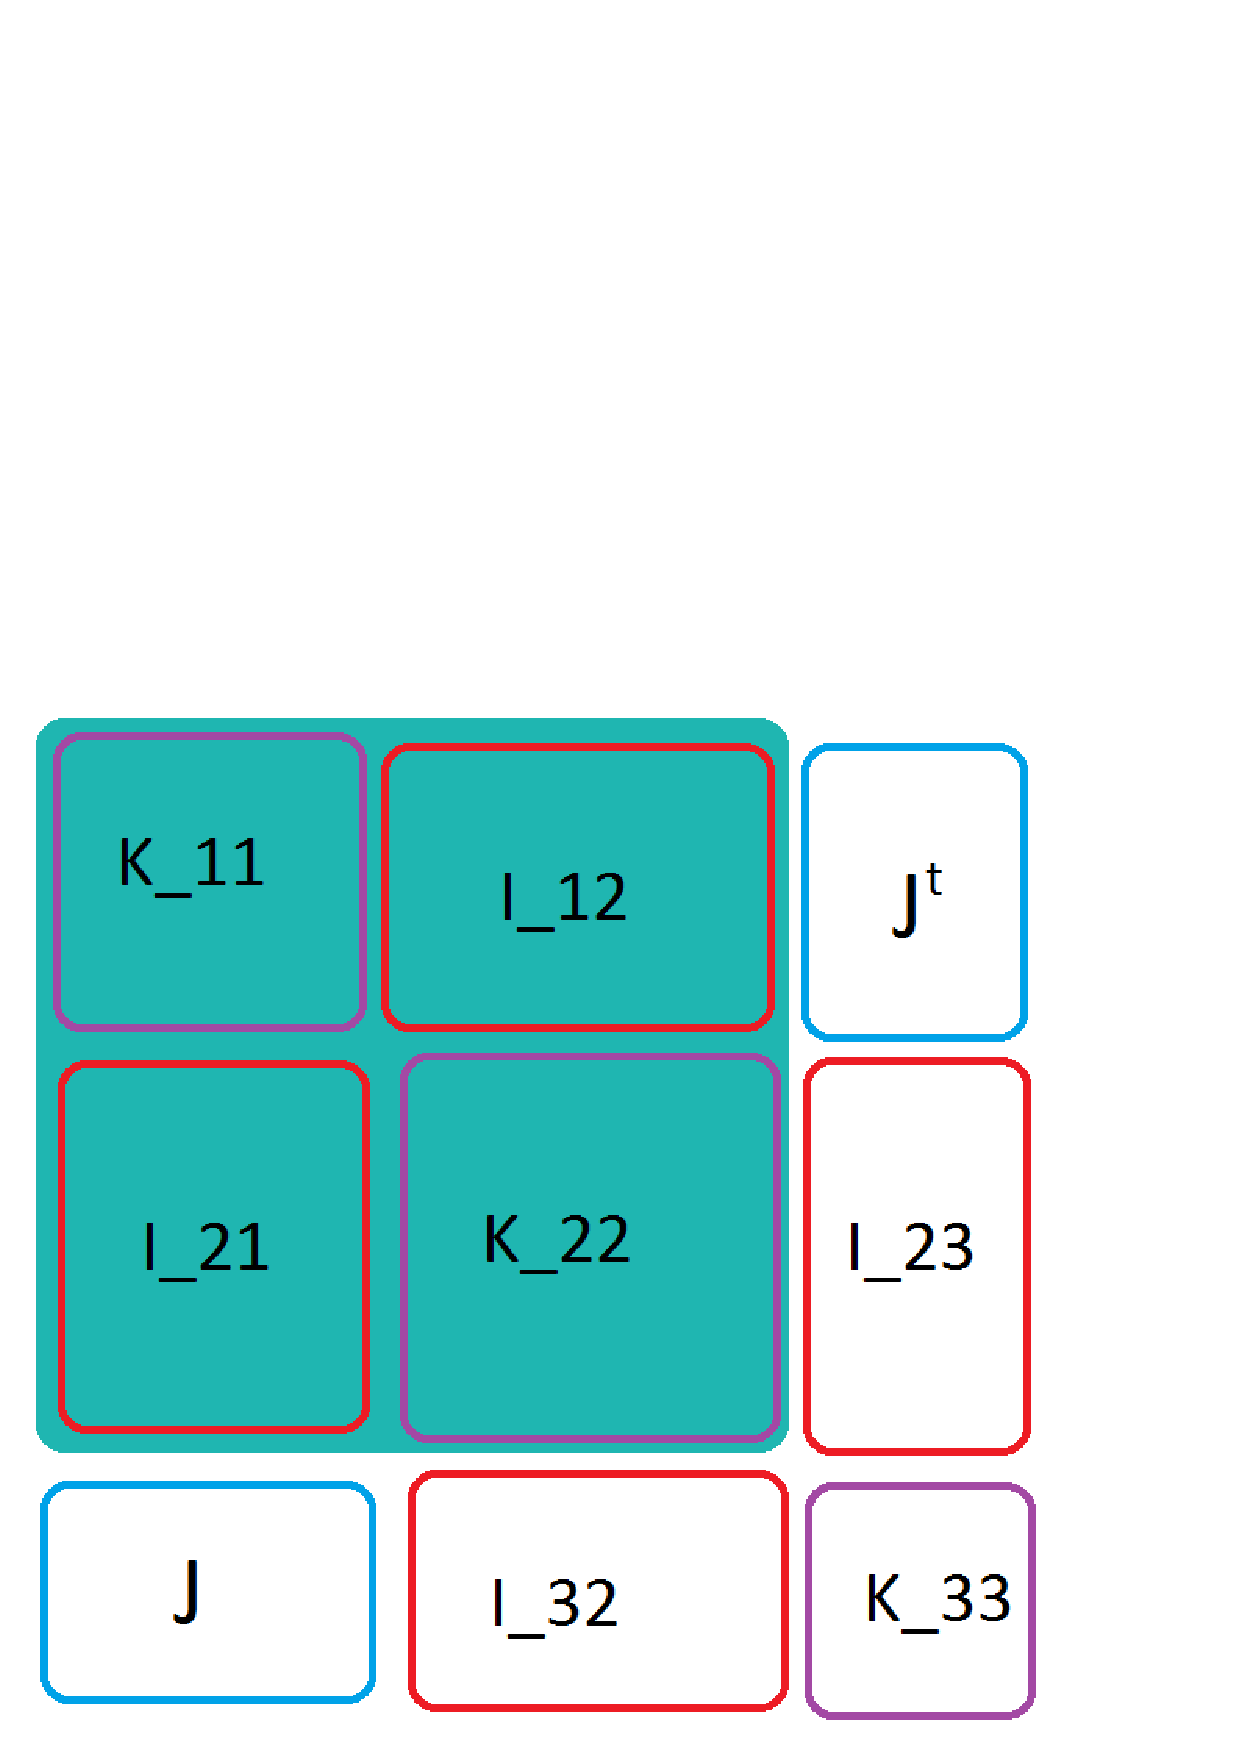
\includegraphics[scale=0.3]{interaction_Real_Mapped_Matrix}        
& 
\includegraphics[scale=0.35]{interaction_Real_Mapped} 
\end{array}
\]
In the case where one of the two mechanical states in interaction is non-mapped, the propagation can be computed directly by the formula :
\[
\left\{ 
\begin{array}{ll}
K_{11}       & += J^t * K_{33} * J               \\
\text{or,}   &                                   \\
K_{tempo}    & =  J^t * K_{33}                   \\
K_{11}       & += K_{tempo} * J                  \\ 
\text{and,}&                 \\      
I_{12}       & += J^t * I_{32}                   \\ 
I_{21}       & += I_{23} * J                        
\end{array}
\right.
\]
\paragraph{Interaction beweent Mapped Mechanical Object and Mapped Mechanical Object}
\begin{center}
  \includegraphics[scale=0.3]{interaction_Mapped_Mapped}
\end{center}
In the case where the two mechanical states in interaction are mapped, the propagation can be computed by two steps. The first consist to propagate the interaction $I_{34}$ to the interation $I_{14}$ :
\[
\left\{ 
\begin{array}{ll}
K_{11}       & += J^t * K_{33} * J               \\
\text{or,}   &                                   \\
K_{tempo}    & =  J^t * K_{33}                   \\
K_{11}       & += K_{tempo} * J                  \\ 
\text{and,}&                 \\      
I_{14}       & += J^t_A * I_{34}                  \\ 
I_{41}       & += I_{43} * J_A                        
\end{array}
\right.
\]
The following step can compute as the one of above paragraph, propagating the interation $I_{14}$ to $I_{12}$.


%In summary, ODE solution is performed using a hierarchy of algorithms and data structures with each level implemented in a different component: the main ODE solution algorithm , the auxiliary linear solver  parameterized by the type of matrix, and an optional preconditioner when the Conjugate Gradient linear solver is used.
%Using a direct solver requires the explicit computation and storage of the system matrix \mat A of Equation~\ref{eq:linear-system}.
%The mass and stiffness matrices are written by the components and summed at each node level. They are then multiplied by the projection and mapping matrices during visitor traversals, and stored in the solver.

\section{Constraint solvers} 
\label{lm}
To handle different kinds of interactions (contact, friction, joints between particles..) between the simulated objects, SOFA allows the use of Lagrange multipliers~\cite{DDKA06}. 
%see \textit{e.g.}\cite{Duriez_eurographics2008}.
%The third family of solvers involves non-trivial constraints requiring additional equations, and additional unknowns called 
They may be combined with explicit or implicit integration.
Each constraint depends on the relative position of the interacting objects, and on optional parameters 
(such as a friction coefficient, etc.)\footnote{For simplicity, we present the equations for two interacting objects 
(rigid or deformable) $1$ and $2$, but the solution applies to arbitrary number of interacting bodies.}:
\begin{equation}
\begin{array}{c}
\Phi(\Vx_1, \Vx_2, ...) = 0 \\ 
\Psi(\Vx_1, \Vx_2, ... ) \geq 0
\end{array}
\label{eq:constraints}
\end{equation} where $\Phi$ represents the bilateral interaction laws (attachments, sliding joints, etc.) whereas $\Psi$ represents unilateral interaction laws (contact, friction, etc.). These functions can be non-linear.
% The solution uses Lagrange multipliers and a single linearization by time step (see~\cite{DDKA06}). 
The Lagrange multipliers are computed at each simulation step.
%However, for interaction including deformations, there is often a temporal coherency on the multipliers values. 
%Thus, we can provide an estimate $\tilde{\lambda}$ at the beginning of each time step and compute a correction $\Delta \lambda$ so that $\lambda = \tilde{\lambda} +\Delta \lambda$.  
They add force terms to Equation (\ref{eq:linear-system}):
\begin{equation}
\begin{array}{c}
\mathbf{A}_1  \Vdv_1 = \mathbf{b}_1 + \mathbf{H}_1^T \lambda\\
\mathbf{A}_2  \Vdv_2 = \mathbf{b}_2 + \mathbf{H}_2^T \lambda
\label{eq:constraint-systeme}
\end{array}
\end{equation}
where 
\begin{equation}
\mathbf{H}_1 = [\frac{\delta \Phi}{\delta \Vx_1} \  ; \  \frac{\delta \Psi}{\delta \Vx_1}  ]\qquad  \mathbf{H}_2 = [\frac{\delta \Phi}{\delta \Vx_2} \  ; \  \frac{\delta \Psi}{\delta \Vx_2}  ].
\end{equation}
Matrices $\mathbf{H}_1$ and $\mathbf{H}_2$ are stored in the mechanical state component of each node. Thus, when the constraint applies to a model that is mapped (see section \ref{sec:mappings}), the constraints are recursively mapped upward like forces to be applied to the independent degrees of freedom~\cite{Duriez_eurographics2008}. 
% An example that illustrates this concept can be found in \cite{Duriez_eurographics2008}. 
Solving the constraints is done by following these steps:


\textbf{Step 1, Free Motion}: interacting objects are solved independently while setting $ \lambda  = 0$. 
We obtain what we call a \textit{free motion} $\Vdv_1^{\mathrm{f}}$  and  $\Vdv_2^{\mathrm{f}}$ for each object. After integration, we obtain $\Vx_{1}^{\mathrm{f}}$ and $\Vx_{2}^{\mathrm{f}}$. 
%For the prediction, use $\tilde{\lambda} = \lambda^{t}$. 
During this step, each object solves equation~(\ref{eq:constraint-systeme}) with $ \lambda  = 0$ independently using a dedicated solver.  

\vspace{2mm}

\textbf{Step 2, Constraint Solving}: 
%the constraint laws are linearized as follows:
%\begin{equation}
%\label{eq:const-lin}
%\underbrace{
%\left[ \! \! \!
%\begin{array}{c}
%\Phi(\Vx_{1}^{t+h}, \Vx_{2}^{t+h})  \\
%\Psi(\Vx_{1}^{t+h}, \Vx_{2}^{t+h}) 
%\end{array} \! \! \!
%\right]}_{\boldsymbol{\delta}^{t+h}}  \! 
%=  \! 
%\underbrace{
%\left[ \! \! \!
%\begin{array}{c}
%\Phi(\Vx_{1}^{\mathrm{f}}, \Vx_{2}^{\mathrm{f}})  \\
%\Psi(\Vx_{1}^{\mathrm{f}}, \Vx_{2}^{\mathrm{f}}) 
%\end{array}\! \! \!
%\right]}_{\boldsymbol{\delta}^{\mathrm{f}}}
% + h\mathbf{H}_1\Vdv_1^{\mathrm{c}}  +  h\mathbf{H}_2\Vdv_2^{\mathrm{c}}
%\end{equation}
%With $\Vdv_1^{\mathrm{c}}$ and $\Vdv_2^{\mathrm{c}}$ being the unknown corrective motion ($\Vdv= \Vdv^{\mathrm{f}} + \Vdv^{\mathrm{c}}$) when solving equation \ref{eq:constraint-systeme} with $\mathbf{b}_1 = \mathbf{b}_2 = 0$. By gathering equations \ref{eq:constraint-systeme} and \ref{eq:const-lin}, we have:
The constrained equations can be linearized and linked to the dynamics (see \cite{CJADLC10} for details). 
\begin{equation}
\left[
\begin{array}{c}
\Phi(\Vx_{1}, \Vx_{2})  \\
\Psi(\Vx_{1}, \Vx_{2}) 
\end{array} \! \! \!
\right]
 =
 % \underbrace{
\left[ \! \! \!
\begin{array}{c}
\Phi(\Vx_{1}^{\mathrm{f}}, \Vx_{2}^{\mathrm{f}})  \\
\Psi(\Vx_{1}^{\mathrm{f}}, \Vx_{2}^{\mathrm{f}}) 
\end{array}\! \! \!
\right]
%}_{ \delta^{\mathrm{f}}  }
 + 
 \underbrace{
 h\mathbf{H}_1\Vdv_1^{\mathrm{c}}  +  h\mathbf{H}_2\Vdv_2^{\mathrm{c}}
 }_{h \left[  \mathbf{H}_1 \mathbf{A}_1^{-1}  \mathbf{H}_1^T + \mathbf{H}_2 \mathbf{A}_2^{-1}  \mathbf{H}_2^T \right]\lambda
 }
 %=
 %\delta^{\mathrm{f}} +
%\underbrace{h \left[  \mathbf{H}_1 \mathbf{A}_1^{-1}  \mathbf{H}_1^T + \mathbf{H}_2 \mathbf{A}_2^{-1}  \mathbf{H}_2^T \right]}_{\mathbf{W}} \lambda
\label{eq:addjminvjt}
\end{equation}
With $\Vdv^{\mathrm{c}} = \Vdv - \Vdv^{\mathrm{f}}$. 
Together with equation (\ref{eq:constraints}), these equations compose a Mixed Complementarity Problem that can be solved by a variety of solvers.
We compute the value of $ \lambda$ using a projected Gauss-Seidel algorithm that iteratively checks and projects the various constraint laws contained in $\Phi$ and  $\Psi$ ~\cite{DGMCG09}. 

\textbf{Step 3, Corrective Motion}: when the value of $\lambda$ is available, the corrective motion is computed as follows:
%
\begin{equation}
\label{eq:corrective-motion}
\begin{array}{c}
\Vx_{1}^{t+h} =  \Vx_{1}^{\mathrm{f}} + h \Vdv_1^{\mathrm{c}} \  \  \mathrm{ with } \  \  \Vdv_1^{\mathrm{c}} = \mathbf{A}_1^{-1}  \mathbf{H}_1^T \lambda \\
\Vx_{2}^{t+h} =  \Vx_{2}^{\mathrm{f}} + h \Vdv_2^{\mathrm{c}} \  \  \mathrm{ with } \  \  \Vdv_2^{\mathrm{c}} = \mathbf{A}_2^{-1}  \mathbf{H}_2^T \lambda
\end{array}
\end{equation}
%

A Master Solver, which is generally placed at the top of the graph of SOFA has the role of imposing this new scheduling to the rest of the graph. 
%
\begin{figure}[!htb]
\centering
% FreeMotionScheme is missing from SVN
\includegraphics[width= 0.9\columnwidth]{ConstraintSolver.png}
\caption{Contact process using constraints: A unilateral constraint is placed at the level of the contact points. The constraint direction is mapped to the degrees of freedom of the objects to obtain matrix $ \mathbf{H}^T$. The \textit{ConstraintCorrections} components compute the compliance to obtain equation \ref{eq:addjminvjt}. The Constraint solver found a new value of $\lambda$ which is sent to the  \textit{ConstraintCorrections} to compute an adequate corrective motion. The Master Solver is placed at the root of the simulation graph to impose the steps of the simulation process.  }
\label{shema_ToH}
\end{figure}

\textbf{Compliance computation} : Equations~\ref{eq:addjminvjt} and~\ref{eq:corrective-motion} involve the inverse of matrix $\mathbf{A}$ (called compliance matrix), which changes at every time step namely in case of a non-linear model. 
Depending on the simulation case, computing this inverse could be time consuming for real-time simulation. 
When this is too time-consuming, we propose several strategies to improve the speed of the algorithm such as using the diagonal of $\mathbf{A}$ instead of the hole matrix, or a precomputed inverse~\cite{Saupin08}, or an asynchronous factorization on the GPU~\cite{CourtecuisseMICCAI11}.  
These strategies are implemented in a category of components, called  \textit{ConstraintCorrections} that provide different ways of computing $\Vdv^{\mathrm{c}}$ given a value of $\lambda$. Given a simulation, it is very easy to make tests and chose the better solution.




